\begin{figure*}[t]
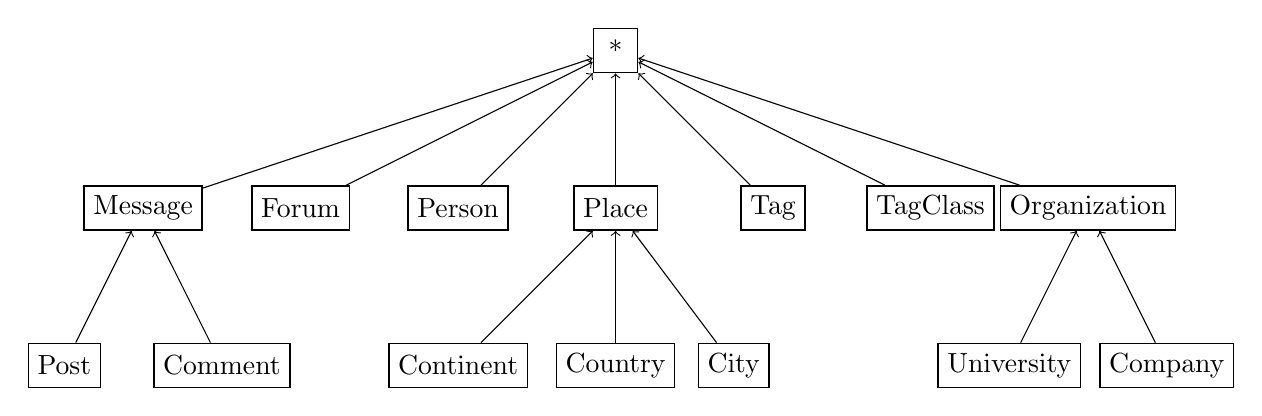
\begin{tikzpicture}
\node[draw=black,minimum size = 16pt,line width = 0.5pt,] at (0, 0)  		(ROOT)	{*};
\node[draw=black,minimum size = 16pt,line width = 0.5pt,] at (-6, -2) 	(N1) 	{Message};
\node[draw=black,minimum size = 16pt,line width = 0.5pt,] at (-4, -2) 	(N2)	{Forum};
\node[draw=black,minimum size = 16pt,line width = 0.5pt,] at (-2, -2) 	(N3) 	{Person};
\node[draw=black,minimum size = 16pt,line width = 0.5pt,] at (0, -2)  	(N4) 	{Place};
\node[draw=black,minimum size = 16pt,line width = 0.5pt,] at (2, -2)  	(N5) 	{Tag};
\node[draw=black,minimum size = 16pt,line width = 0.5pt,] at (4, -2)  	(N6) 	{TagClass};
\node[draw=black,minimum size = 16pt,line width = 0.5pt,] at (6, -2)  	(N7)	{Organization};
\node[draw=black,minimum size = 16pt,line width = 0.5pt,] at (-7, -4) 	(N11) 	{Post};
\node[draw=black,minimum size = 16pt,line width = 0.5pt,] at (-5, -4) 	(N12) 	{Comment};
\node[draw=black,minimum size = 16pt,line width = 0.5pt,] at (-2, -4)  	(N41) 	{Continent};
\node[draw=black,minimum size = 16pt,line width = 0.5pt,] at (0, -4)  	(N42) 	{Country};
\node[draw=black,minimum size = 16pt,line width = 0.5pt,] at (1.5, -4)  	(N43) 	{City};
\node[draw=black,minimum size = 16pt,line width = 0.5pt,] at (5, -4)  	(N71)	{University};
\node[draw=black,minimum size = 16pt,line width = 0.5pt,] at (7, -4)  	(N72)	{Company};
\draw[<-] (ROOT) -- (N1);
\draw[<-] (ROOT) -- (N2);
\draw[<-] (ROOT) -- (N3);
\draw[<-] (ROOT) -- (N4);
\draw[<-] (ROOT) -- (N5);
\draw[<-] (ROOT) -- (N6);
\draw[<-] (ROOT) -- (N7);
\draw[<-] (N1) -- (N11);
\draw[<-] (N1) -- (N12);
\draw[<-] (N4) -- (N41);
\draw[<-] (N4) -- (N42);
\draw[<-] (N4) -- (N43);
\draw[<-] (N7) -- (N71);
\draw[<-] (N7) -- (N72);
\end{tikzpicture}
\caption{Label hierarchy for the SNB database.}
\end{figure*} 
